\documentclass{beamer}

\usepackage[ngerman]{babel}
\usepackage{epstopdf}
\usepackage{bibgerm}
\usepackage[T1]{fontenc}
\usepackage[utf8]{inputenc}
\usepackage{ifthen}
\usepackage{graphicx}
\usepackage{fancyvrb}
\newcommand*{\fvr}[1]{\textcolor{red}{#1}}
\newcommand*{\fvb}[1]{\textcolor{blue}{#1}}
\newcommand*{\fvp}[1]{\textcolor{purple}{#1}}

\setbeamertemplate{navigation symbols}{}
\setbeamertemplate{footline}[frame number]

\title{salbnet für DNS}
\subtitle{Implementation und Messung}
\author{Sebastian Menski\\menski@uni-potsdam.de}
\institute{Institut für Informatik\\Universität Potsdam}
\date{09. Mai 2012}

\begin{document}

  \frame{\thispagestyle{empty}\titlepage}
  \frame{\thispagestyle{empty}\frametitle{Gliederung}\tableofcontents{}}

  \newcommand{\mytitle}{}

  \newcommand{\mysection}[1]{
    \renewcommand{\mytitle}{#1}
    \section{#1}
    \frame{\thispagestyle{empty}
      \begin{center}
        \textcolor{beamer@blendedblue}{\LARGE\mytitle}
      \end{center}
    }
  }

  \newcommand{\myframe}[2][\empty]{
    \frame{\frametitle{\mytitle}
      \ifthenelse{\equal{#1}{\empty}}
      {#2}
      {\framesubtitle{#1}#2}
    }
  }

  \newcommand{\mybreakframe}[2][\empty]{
    \frame[allowframebreaks]{\frametitle{\mytitle}
      \ifthenelse{\equal{#1}{\empty}}
      {#2}
      {\framesubtitle{#1}#2}
    }
  }

	\mysection{Rückblick}
	
	\myframe[Was ist salbnet?]{
		\small{
		\begin{quote}
The load balancing in salbnet is application indepedent and credit based. Backend server report
credits to the load balancer. The credits represent the maximum number of requests which a backend
server is able to handle.\footnote{\url{http://salbnet.org}}
		\end{quote}}
		\begin{columns}
		\column{3cm}
		
\includegraphics[width=3cm]{images/logo.png}
	\column{7cm}
		Komponenten von salbnet:
		\begin{itemize}
			\item	libnethook
			\item libnetmsg
			\item salbd
			\item servload
		\end{itemize}
	\end{columns}
	}

	\myframe[DNS Erweiterung] {
		\begin{itemize}
			\item servload soll DNS-Pakete versenden
			\item salbd berechnet Credits für den BIND Server
			\item Kommunikation von salbd über TCP/IP (optional)
		\end{itemize}
	}

	\mysection{Konzept}

	\myframe{
		\begin{itemize}
			\item servload liest BIND Log-Datei und baut DNS-Pakete
			\item servload sendet DNS-Anfragen an Load Balancer
			\item salbd (Server) verteilt Last nach gemeldeten Credits
			\item salbd (Client) misst Last des BIND-Servers
		\end{itemize}
	}

	\mysection{Implementierung}

	\myframe{
		\begin{itemize}
			\item servload: Implementierung nach RFC1035
			\item libnetmsg: Vervollständigung der ungetesten TCP-Kommunikation
			\item salbd (Client): ermitteln der Metriken
				\begin{itemize}
					\item Größe der UDP-Receive-Queue (\texttt{/proc/sys/net/core/rmem\_default})
					\item Aktueller Füllstand der UDP-Receive-Queue (\texttt{/proc/net/udp})
					\item Drops (\texttt{/proc/net/snmp})
					\item Median der empfangenen Paketgrößen (\texttt{recvmsg}) 
				\end{itemize}
			\item libnethook: Abfangen des \texttt{recvmsg} Aufrufs von BIND
		\end{itemize}
	}

	\myframe[Problem Paketgröße]{
		\begin{itemize}
			\item \texttt{recvmsg} liefert größe der DNS-Nachricht zurück
			\item entspricht nicht Größe der Nachricht in der Receive-Queue
			\item Daten werden mit \texttt{struct sk\_buff} organisiert
		\end{itemize}
	}

	\myframe[(Lokale) Lösung] {
		\begin{itemize}
			\item Vorgehen:
				\begin{itemize}
					\item Senden von UDP-Paketen mit steigender Größe
					\item Größe des UDP-Pakets in der Receive-Queue ermitteln
					\item Paket mit \texttt{recvmsg} abholen
					\item Zusammenhang zwischen den Größen herstellen und Formel entwickeln
				\end{itemize}
		\end{itemize}
	}

	\myframe[(Lokale) Lösung] {
		\begin{table}
			\centering
			\begin{tabular}{cc}
			Receive-Queue & recvmsg \\\hline
			376 & 12-64	\\
			504 & 65-192	\\
			632 & 193-320	\\
			760 & 321-448 \\
			888 &	449-576\\
			\end{tabular}
			\caption{Beobachtung}
		\end{table}
		\begin{equation*}
			\text{Receive-Queue} = \lfloor (recvmsg + 63) / 128 \rfloor * 128 + 376
		\end{equation*}
	}

	\myframe[Credit Berechnung] {
		\begin{equation*}
			Credits = \frac{\text{Größe der Receive-Queue} - \text{Aktueller Füllstand}}{\text{Median der
	Paketgröße}}
		\end{equation*}
	}

	\mysection{Messung}
		
	\myframe[Messumgebung]{
		\begin{itemize}
			\item servload auf node015 vom Leibniz-Cluster (12GB RAM)
			\item LVS + salbd (Server) auf ib1 vom IB-Cluster (2x AMD Opteron 244 @ 1,8GHz)
			\item BIND + salbd (Client) auf ib4, ib6 und ib8 vom IB-Cluster
				\begin{itemize}
					\item ib4: 2x AMD Opteron 244 @ 1,8GHz
					\item ib6: 1x Intel Pentium 4 @ 2,8GHz
					\item ib8: 2x Intel Xenon 3040 @ 1,8Ghz
				\end{itemize}
			\item UDP-Receive-Queue: 24MB (Standard: 126 kb)
		\end{itemize}
	}

	\myframe[Testablauf] {
		\begin{itemize}
			\item wrr vs. salbd (dpr)
			\item Gewichte: ib4$\rightarrow$788  ib6$\rightarrow$623 ib8$\rightarrow$1181 (UnixBench)
			\item Log: 5min (29-Sep-2011 5:55:00-6:00:00)
			\item Verstärkung: modify 400, 800, 1600
			\item je 51 Durchläufe
		\end{itemize}
	}

	\myframe[BIND-Log] {
			\begin{figure}
				\centering
				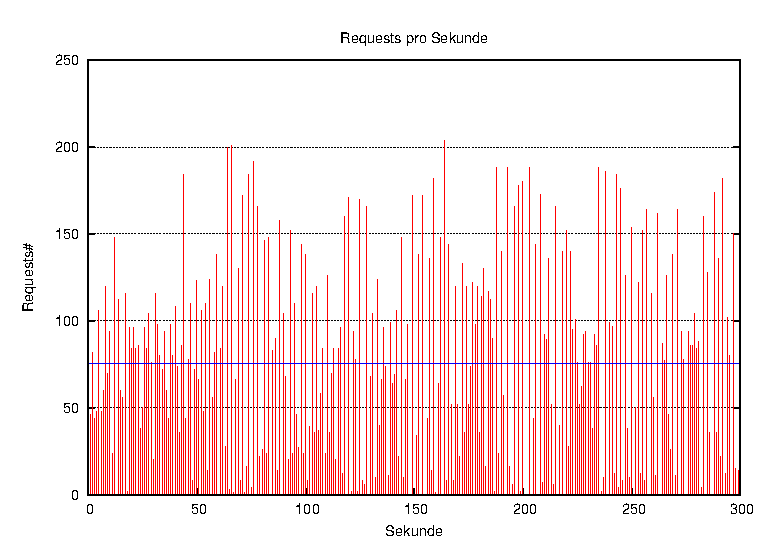
\includegraphics[width=10cm]{plots/requests}
				\caption{Log vom 29-Sep-2011 5:55-6:00}
			\end{figure}
		}

		\myframe[BIND-Log]{ 
			\begin{tabular}{lrrrr}
				Faktor & Requests & Sessions & avg Req/s & max Req/s \\\hline
				1 & 22.594 & 33 & 75,31 & 204 \\
				400 & 9.037.600 & 13.200 & 30.125,33 & 81.600 \\
				800 & 18.075.200 & 26.400 & 60.250,67 & 163.200 \\
				1600 & 36.150.400 & 52.800 & 120.501,33 & 326.400 \\
			\end{tabular}
	}

	\myframe[Ergebnisse] {
		\begin{figure}
			\centering
			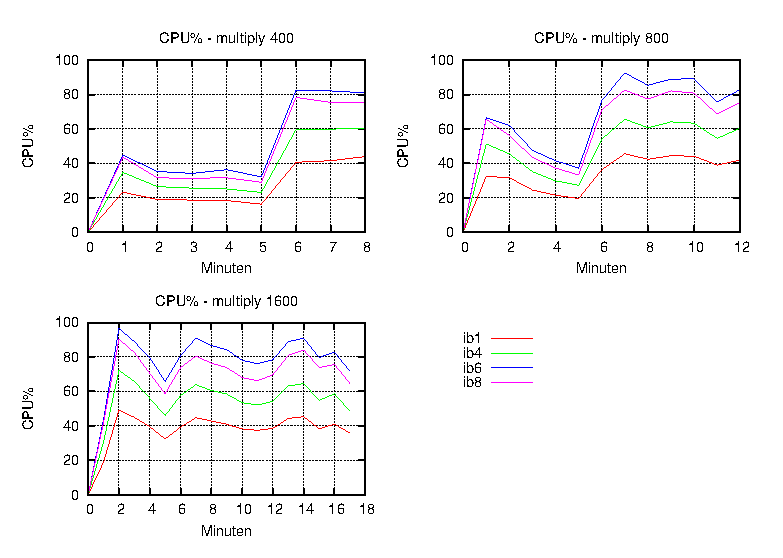
\includegraphics[width=10cm]{plots/cpu}
			\caption{CPU\% IB-Cluster}
		\end{figure}
	}

	\myframe[Ergebnisse] {
		\begin{figure}
			\centering
			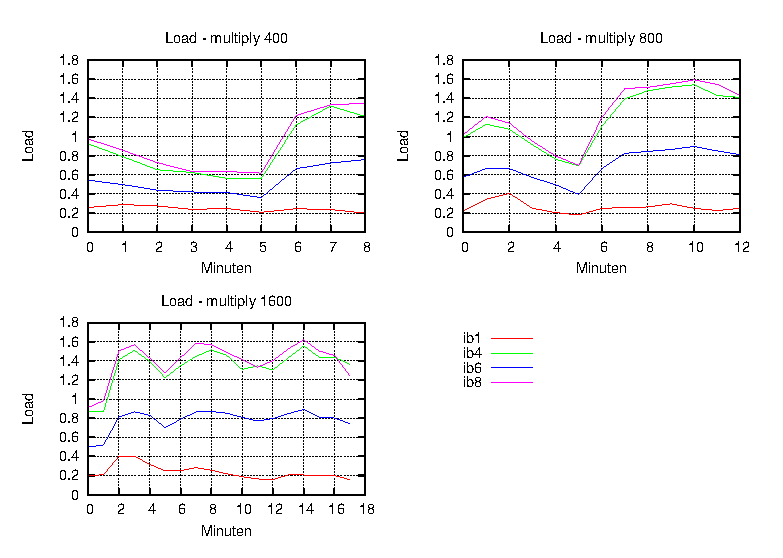
\includegraphics[width=10cm]{plots/load}
			\caption{Load IB-Cluster}
		\end{figure}
	}

	\myframe[Ergebnisse] {
		\begin{figure}
			\centering
			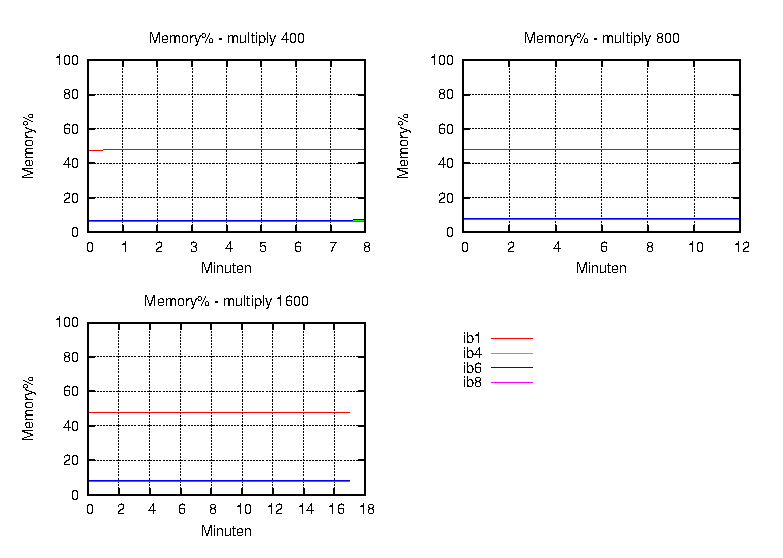
\includegraphics[width=10cm]{plots/memory}
			\caption{Memory\% IB-Cluster}
		\end{figure}
	}

	\myframe[Ergebnisse] {
		\begin{figure}
			\centering
			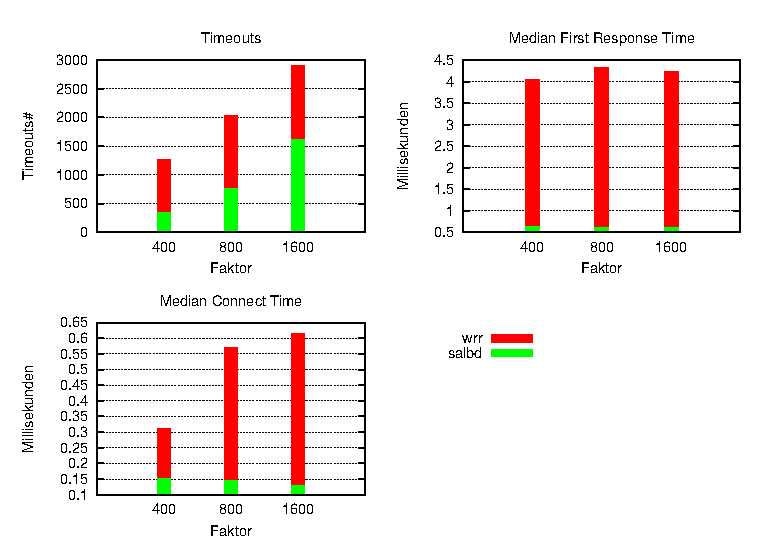
\includegraphics[width=10cm]{plots/servload}
			\caption{Servload Statistiken}
		\end{figure}
	}

	\myframe[Ergebnisse] {
		\begin{table}
			\centering
			\begin{tabular}{r|cc|cc|cc}
				& \multicolumn{2}{c}{multiply 400}
				& \multicolumn{2}{c}{multiply 800}
				& \multicolumn{2}{c}{multiply 1600} \\
				& wrr & salbd & wrr & salbd	& wrr & salbd \\\hline
			TO & 1273,39 & 343,16 & 2038,53 & 759,86 & 2910,16 & 1612,78 \\
		  RT & 4,05& 0,64 & 4,33 & 0,61 & 4,24 & 0,60 \\
			CT & 0,31& 0,15 & 0,57 & 0,14 & 0,61 & 0,13\\
			\end{tabular}
		\end{table}
	}

\end{document}
